\begin{figure}[h]
    \centering
    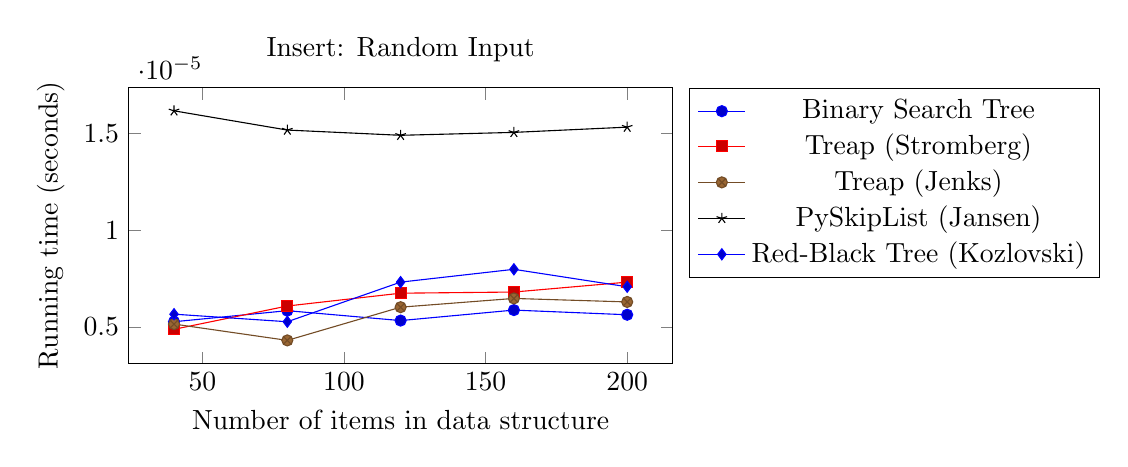
\begin{tikzpicture}
        \begin{axis}[
            xlabel={Number of items in data structure},
            ylabel={Running time (seconds)},
            title={Insert: Random Input},
            width=0.7\textwidth,
            height=2in,
            legend pos=outer north east
        ]
		\addplot coordinates {
			(40, 5.2705683931564275e-06)
			(80, 5.842801532982e-06)
			(120, 5.3308034605042964e-06)
			(160, 5.872919066657323e-06)
			(200, 5.631978797254744e-06)
		};
		\addplot coordinates {
			(40, 4.879040455377237e-06)
			(80, 6.083741802384579e-06)
			(120, 6.7463275432361195e-06)
			(160, 6.806562610586764e-06)
			(200, 7.318560683067244e-06)
		};
		\addplot coordinates {
			(40, 5.1500982584523625e-06)
			(80, 4.306807315548889e-06)
			(120, 6.023506735033934e-06)
			(160, 6.4752697401609934e-06)
			(200, 6.2945645381090595e-06)
		};
		\addplot coordinates {
			(40, 1.6173115583564823e-05)
			(80, 1.5179236972284738e-05)
			(120, 1.4908179169206837e-05)
			(160, 1.5058766837583449e-05)
			(200, 1.5329824640661348e-05)
		};
		\addplot coordinates {
			(40, 5.662096330932842e-06)
			(80, 5.2705683931564275e-06)
			(120, 7.318560683067244e-06)
			(160, 7.981146423918783e-06)
			(200, 7.077620413664665e-06)
		};
        \legend{Binary Search Tree, Treap (Stromberg), Treap (Jenks), PySkipList (Jansen), Red-Black Tree (Kozlovski)}
        \end{axis}
    \end{tikzpicture}
    \caption{Average of 10 operations, benchmarked every 40, starting at 40.}
\end{figure}